\documentclass[a4paper]{article}
\usepackage[margin=1in]{geometry} % 设置边距,符合Word设定
\usepackage{ctex}
\usepackage{graphicx} %插入图片的宏包
\usepackage{float} %设置图片浮动位置的宏包
\usepackage{subfigure} %插入多图时用子图显示的宏包
\usepackage{lipsum}
\usepackage{minted}% 语法高亮和代码样式设置方面更加强大和灵活
\usepackage{listings}% 引入listings包,用于在文档中插入代码,并可自定义代码样式
\title{ This is a test for vscode}
\author{ Ali}
\date{\today}

\begin{document}
    \maketitle
\begin{abstract}
    \lipsum[150]
\end{abstract}
\tableofcontents
\section{Introduction}
\subsection{Background}
\subsection{Our Work}
\subsection{Data Pre-processing}


\section{Assumptions}
我们通过在网上查找多方面的资料并参考权威数据,最后对33个项目的七个维度进行了评分,结果如下:

展示表格

\section{Abbreviation and Definitions}
\section{The Evaluate Model}
\subsection{线性拟合模型}
我们首先排除了一些数据比较差的项目,比如1,2,3.最后我们选择33个项目的数据训练我们的模型。
然后,我们使用一次线性拟合,对每一个项目从1948到2020年的项目数进行了拟合:
\begin{figure}[H] %H为当前位置,!htb为忽略美学标准,htbp为浮动图形
    \centering %图片居中
    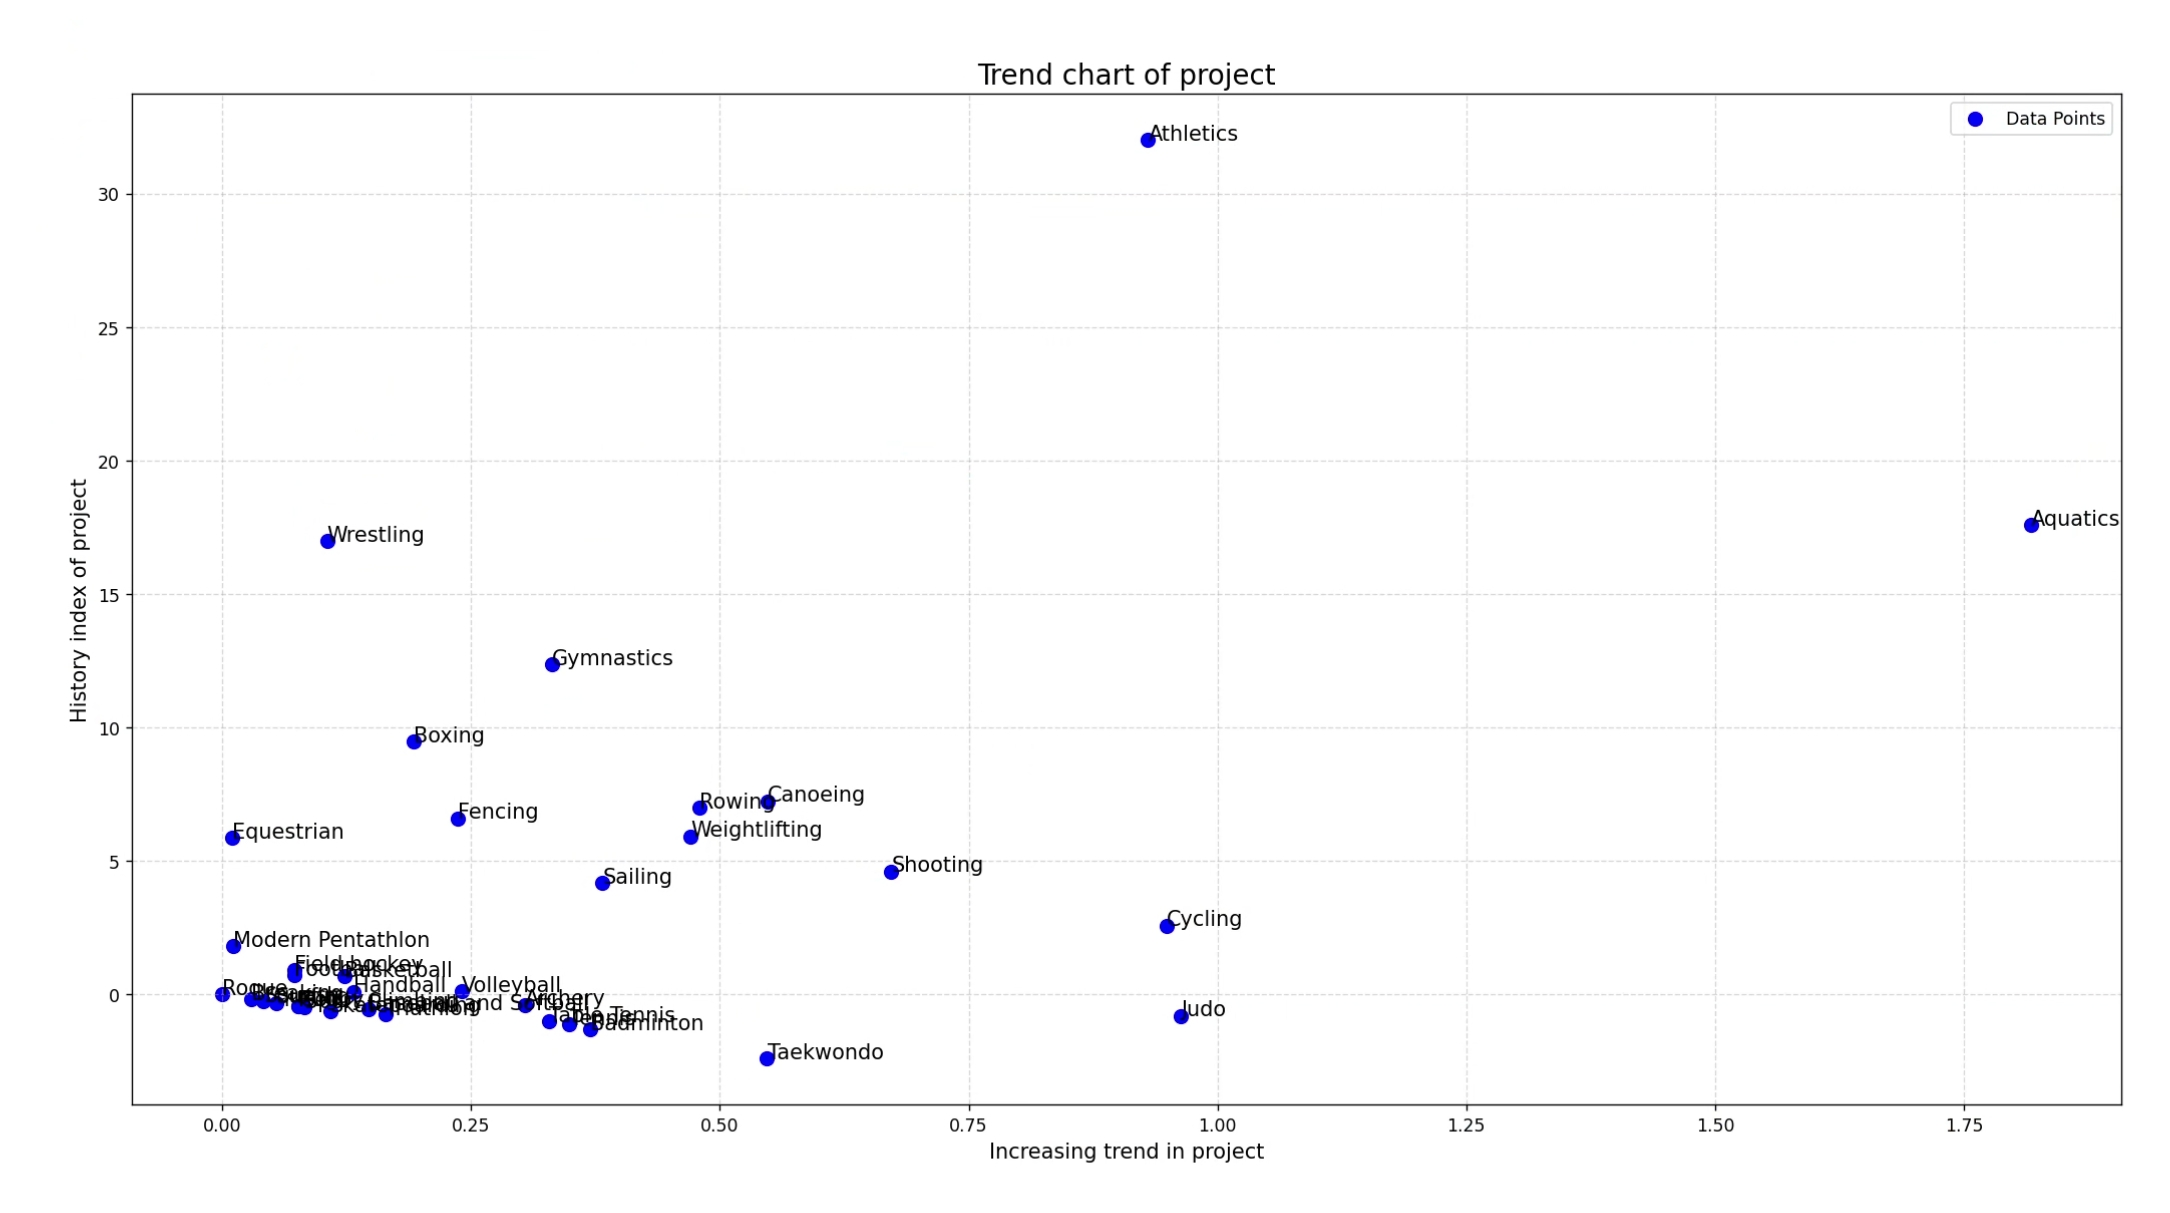
\includegraphics[width=0.7\textwidth]{TrendChartOfProject} %插入图片,[]中设置图片大小,{}中是图片文件名
    \caption{Main name 2} %最终文档中希望显示的图片标题
    \label{Fig.main2} %用于文内引用的标签
    \end{figure}

\subsection{随机森林回归}
\subsubsection{Introduction}
%TODO: 随机森林回归的定义

我们以七个维度和作为自变量,线性拟合的斜率作为因变量,训练了一个随机森林回归模型。

\subsubsection{Implementation}
我们使用了python 的sklearn模块的随机森林拟合算法,
% 行间代码例子
\begin{listing}[htb]
	\caption{处理请求}
	\label{code:processdweet}
	\begin{minted}{python3}
        X = data.iloc[:, :-1]  # 自变量
        y = data.iloc[:, -1]   # 因变量
        X_train, X_test, y_train, y_test = train_test_split(X, y, test_size=0.2, random_state=42)
        # 3. 数据标准化(如果需要)
        scaler = StandardScaler()
        X_train = scaler.fit_transform(X_train)
        X_test = scaler.transform(X_test)
        # 4. 模型选择与训练
        model = RandomForestRegressor(n_estimators=100, random_state=42)
        model.fit(X_train, y_train)
\end{minted}
\end{listing}


\subsubsection{Result Analysis}
在测试集中,我们的模型的R Square误差达到了0.98,均方误差达到0.004,回归训练比较成功。

\begin{quote}
Mean Squared Error: 0.0004830

R-squared: 0.985916
\end{quote}


我们使用了这个模型预测了在训练集与测试集之外的数据:

展示图片33333

结果表明,我们的模型在预测项目数量的增长上取得了成功。



\section{对SDE项目的预测}
我们对某个SDE项目进行了评分,输入我们的模型,得到了如下结果

我们认为 它的增长是xxx
\subsubsection{Background of This Problem}
\subsection{Efficiency and Robustness}
\section{Sensitivity Analysis}
\section{Strengths and Weaknesses}
\subsection{Strengths}
\subsection{Weaknesses}
\section{Conclusion}
Hello world!test123
\end{document}  